\documentclass{article}
\usepackage{amsmath}
\usepackage{amssymb}
\usepackage{ctex}
\usepackage[margin=2cm]{geometry} % 设置较窄的边距使文档宽一些
\usepackage{multirow} % 支持表格中的多行单元格
\usepackage{graphicx} % 用于插入图片
\usepackage{subcaption} % 支持子标题
\usepackage{float} % 支持 [H] 浮动体选项
\title{\heiti\zihao{2}实验二 R、L、C 串联谐振电路的研究 }
\author{\songti  孙振川  PB23081463 \\
课程号  ME2011.04 }
\date{2025.5.20}
\begin{document}
    \maketitle
    
\begin{abstract}
    \noindent{\textbf{摘要:} 本实验主要研究 R、L、C 串联谐振电路的幅频特性曲线,了解电路发生谐振的条件、特点,掌握电路品质因数(电路 Q 值)的物理意义及其测定方法。实验中通过改变信号源频率,测量电压和电流的波形,找到串联谐振频率,并分析不同频率下电压和电流的变化情况。实验结果表明,R、L、C 串联谐振电路具有良好的选择性和谐振特性。}
    
    \noindent{\textbf{关键词:} RLC 串联谐振电路;幅频特性曲线;谐振频率;品质因数;选择性}
\end{abstract}
\section{引言}

\section{实验目的}
\begin{enumerate}
    \item 学习用实验方法绘制 R、L、C 串联电路的幅频特性曲线。 
    \item 加深理解电路发生谐振的条件、特点,掌握电路品质因数(电路 Q 值)的物理意义及其测定方法。
\end{enumerate}

\section{实验原理}
1.在图 1 所示的 $\mathrm{R} 、 \mathrm{~L} 、 \mathrm{C}$ 串联电路中,当正弦交流信号源的频率 f 改变时,电路中的感抗、容抗随之而变,电路中的电流也随 f 而变。取电阻 R 上的电压 $\mathrm{u}_{\mathrm{o}}$ 作为响应,当输入电压 $u_i$ 的幅值维持不变时,在不同频率的信号激励下,测出 $U_0$ 之值,然后以 $f$ 为横坐标,以 $U_0 / U_i$为纵坐标(因 $\mathrm{U}_{\mathrm{i}}$ 不变,故也可直接以 $\mathrm{U}_{\mathrm{O}}$ 为纵坐标),绘出光滑的曲线,此即为幅频特性曲线,亦称谐振曲线,如图所示。


\begin{figure}[h]
    \centering
    \begin{minipage}[t]{0.48\textwidth}
        \centering
        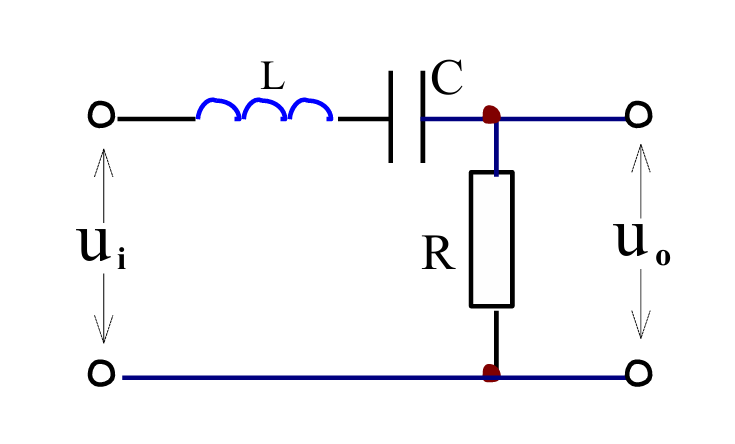
\includegraphics[width=\textwidth]{img1.png}
        \subcaption{串联电路示意图}
        \label{fig:amplitude_frequency_characteristic_1}
    \end{minipage}
    \hfill
    \begin{minipage}[t]{0.48\textwidth}
        \centering
        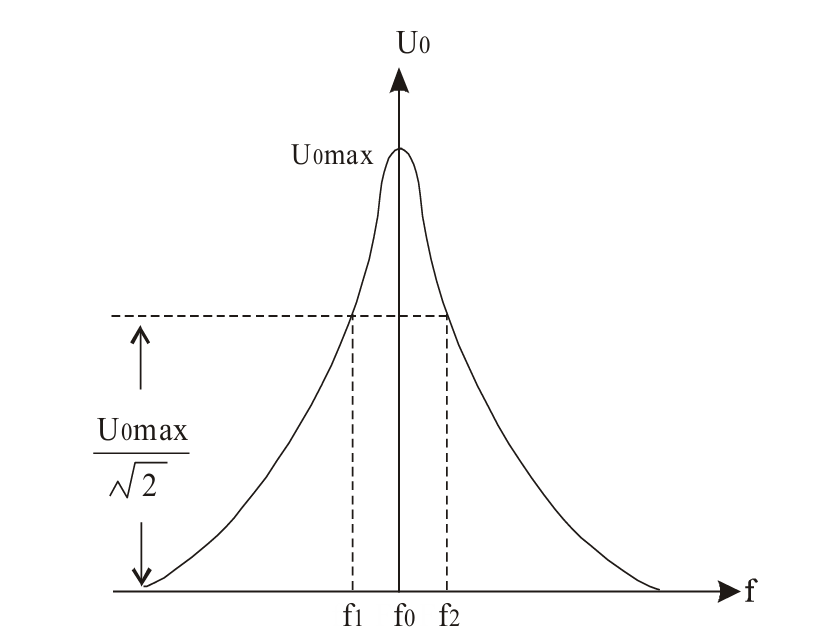
\includegraphics[width=\textwidth]{img2.png}
        \subcaption{幅频特性曲线 2}
        \label{fig:amplitude_frequency_characteristic_2}
    \end{minipage}
    \caption{实验原理}
\end{figure}

2.在 $\mathrm{f}=\mathrm{f}_0=\frac{1}{2 \pi \sqrt{L C}}$ 处,即幅频特性曲线尖峰所在的频率点称为谐振频率。此时 $\mathrm{X}_{\mathrm{L}}=\mathrm{Xc}$ ,电路呈纯阻性,电路阻抗的模为最小。在输入电压 $\mathrm{U}_{\mathrm{i}}$ 为定值时,电路中的电流达到最大值,且与输入电压 $u_i$ 同相位。从理论上讲,此时 $U_i=U_R=U_O, U_L=U_c=Q U_i$ ,式中的 $Q$ 称为电路的品质因数。

3.电路品质因数 Q 值的两种测量方法

一是根据公式 $\mathrm{Q}=\frac{U_L}{U_o}=\frac{U_C}{U_o}$ 测定, $\mathrm{U}_{\mathrm{C}}$ 与 $\mathrm{U}_{\mathrm{L}}$ 分别为谐振时电容器 C 和电感线圈 L 上的电压;

另一方法是通过测量谐振曲线的通频带宽度 $\triangle \mathrm{f}=\mathrm{f}_2-\mathrm{f}_1$ ,再根据 $\mathrm{Q}=\frac{f_O}{f_2-f_1}$ 求出 Q 值。式中 $\mathrm{f}_0$ 为谐振频率, $\mathrm{f}_2$ 和 $\mathrm{f}_1$ 是失谐时,亦即输出电压的幅度下降到最大值的 $1 / \sqrt{2} \quad(=0.707)$ 倍时的上、下频率点。Q 值越大,曲线越尖锐,通频带越窄,电路的选择性越好。在恒压源供电时,电路的品质因数、选择性与通频带只决定于电路本身的参数,而与信号源无关。


\section{实验器材}
\label{sec:equipment}
    \begin{enumerate}
        \item 低频函数信号发生器 
        \item 交流毫伏表
        \item 双踪示波器
        \item 频率计 
        \item HE-15 谐振电路实验电路板 
    \end{enumerate} 

\section{实验内容}
1.利用 HE-15 实验箱上的" $\mathrm{R} 、 \mathrm{~L} 、 \mathrm{C}$ 串联谐振电路",按图 $2$ 组成监视、测量电路。选 $\mathrm{C}_1=0.01 \mu \mathrm{~F}$ 。用交流毫伏表测电压,用示波器监视信号源输出。令信号源输出电压 $\mathrm{U}_{\mathrm{i}}=3 \mathrm{~V}_{\mathrm{P}-\mathrm{P}}$ ,并保持不变。

\begin{figure}[h]
    \centering
    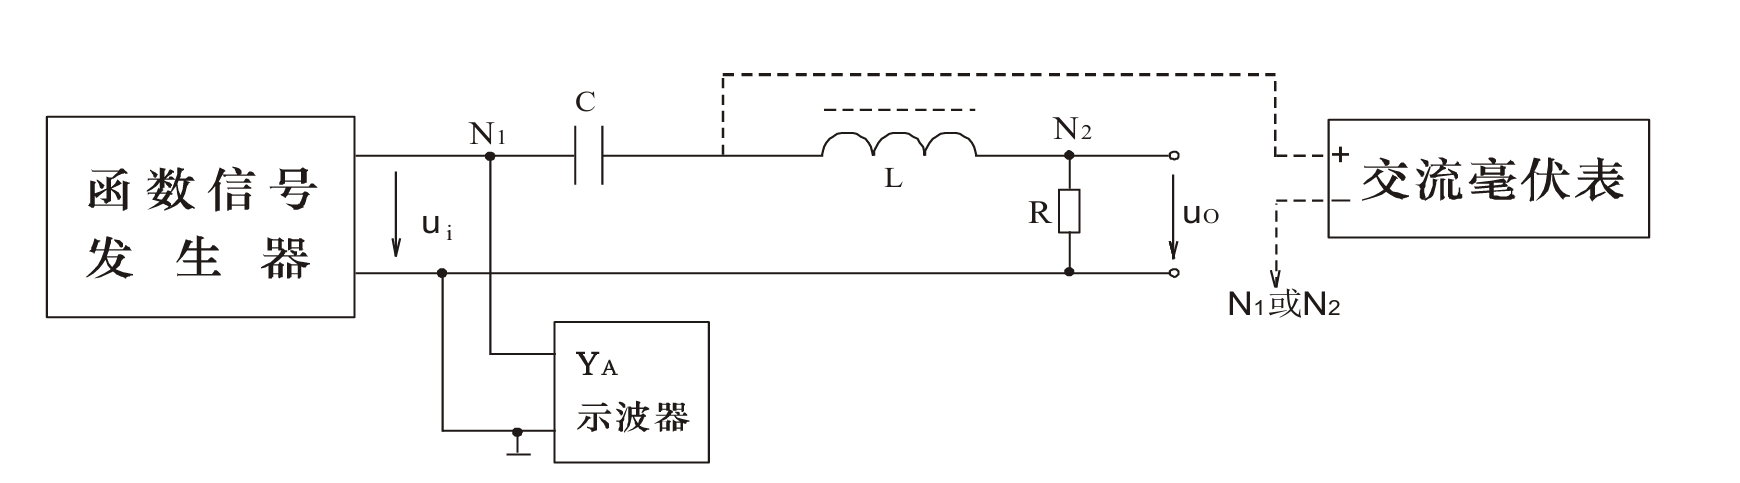
\includegraphics[width=0.8\textwidth]{img3.png}
    \caption{电路示意图}
    \label{fig:diff_circuit}
\end{figure}

2.找出电路的谐振频率 $\mathrm{f}_0$ ,其方法是,将毫伏表接在 $\mathrm{R}(200 \Omega)$ 两端,令信号源的频率由小逐渐变大(注意要维持信号源的输出幅度不变),当 Uo 的读数为最大时,读得频率计上的频率值即为电路的谐振频率 $\mathrm{f}_0$ ,并测量 $\mathrm{U}_{\mathrm{C}}$ 与 $\mathrm{U}_{\mathrm{L}}$ 之值(注意及时更换毫伏表的量限)。

3.在谐振点两侧,按频率递增或递减 $100 \mathrm{~Hz} 、 200 \mathrm{~Hz} 、 500 \mathrm{~Hz}$ 或 1 KHz,依次各取 8 个测量点,逐点测出 $U_O, U_L, U_C$ 之值,记入数据表格。
\subsection{C1 = 0.01µ F, R2 = 200Ω}

\begin{figure}[H]
    \centering
    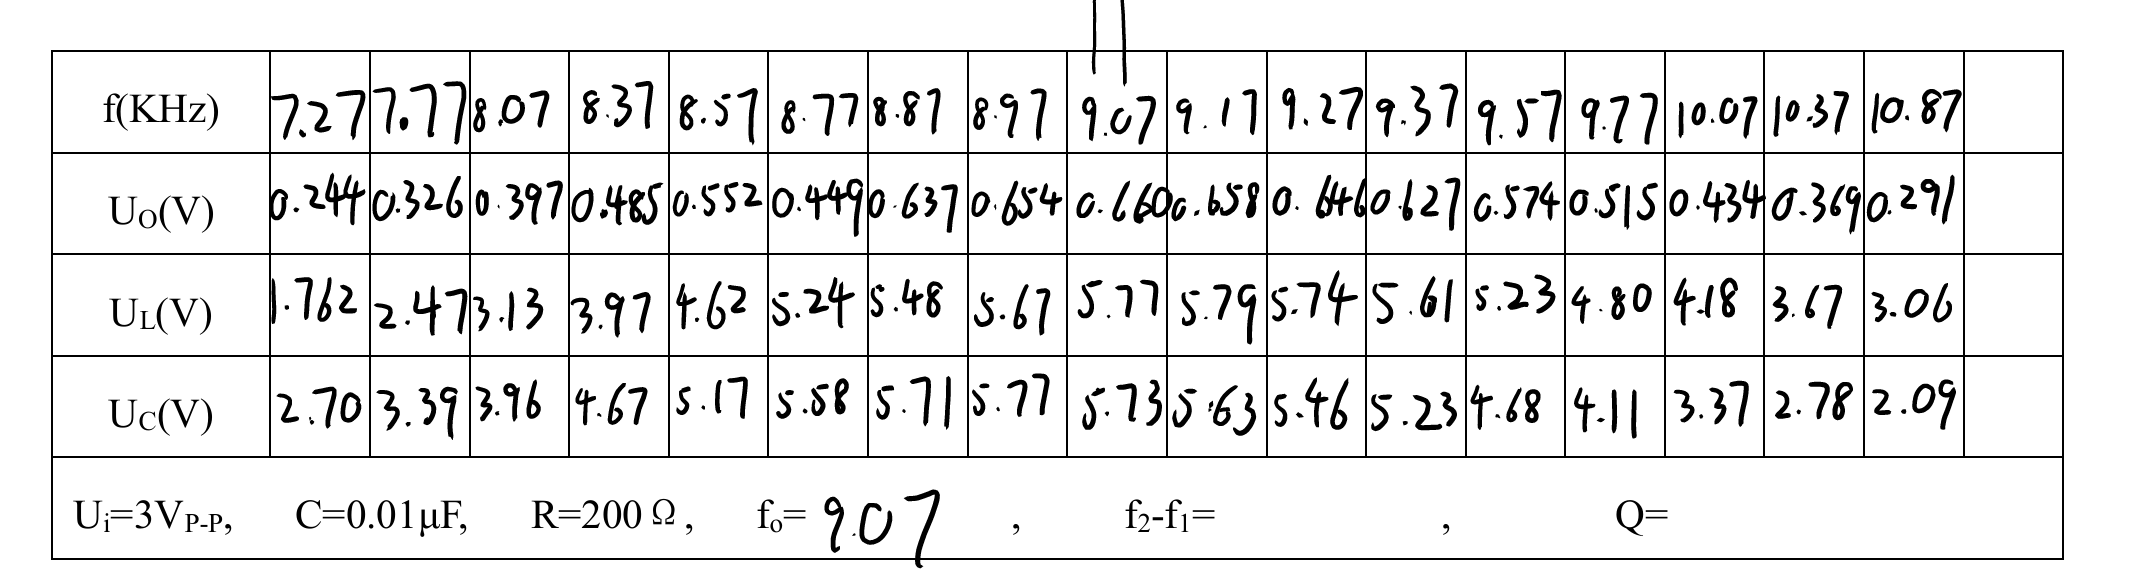
\includegraphics[width=\textwidth]{img4.png}
    \caption{ $\mathrm{C}_1=0.01 \mu \mathrm{~F}, \mathrm{R}_1=200 \Omega$}
    \label{fig:diff_circuit}
\end{figure}

\subsubsection{第一种方法测 Q 值}
根据公式 $\mathrm{Q}=\frac{U_L}{U_o}=\frac{U_C}{U_o}$ 测定, $\mathrm{Q}=\frac{U_L}{U_o}=\frac{U_C}{U_o}=5.77/0.66=8.7$
\subsubsection{通频带宽法 Q 值}
$\mathrm{U}_{\mathrm{i}}=3 \mathrm{~V}_{\mathrm{P}-\mathrm{P}}, \quad \mathrm{C}=0.01 \mu \mathrm{~F}, \quad \mathrm{R}=200\Omega, \quad \mathrm{f}_0=9.06 \mathrm{k}  \mathrm{Hz}$

$f1 = 8.22 \mathrm{kHz}\quad f2 = 10.12\mathrm{kHz} \quad \mathrm{f}_2-\mathrm{f}_1=1.90\mathrm{kHz}\quad \quad \mathrm{Q}= 4.84$

\begin{figure}[H]
    \centering
    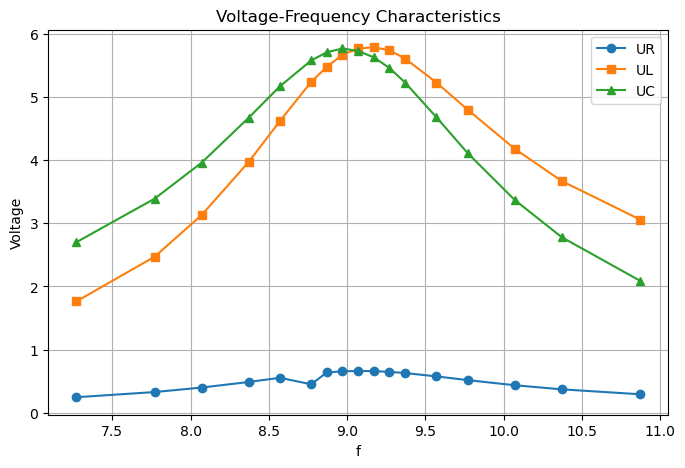
\includegraphics[width=0.8\textwidth]{output.png}
    \caption{ $\mathrm{C}_1=0.01 \mu \mathrm{~F}, \mathrm{R}_1=200 \Omega$}
    \label{fig:diff_circuit}
\end{figure}
\begin{figure}[H]
    \centering
    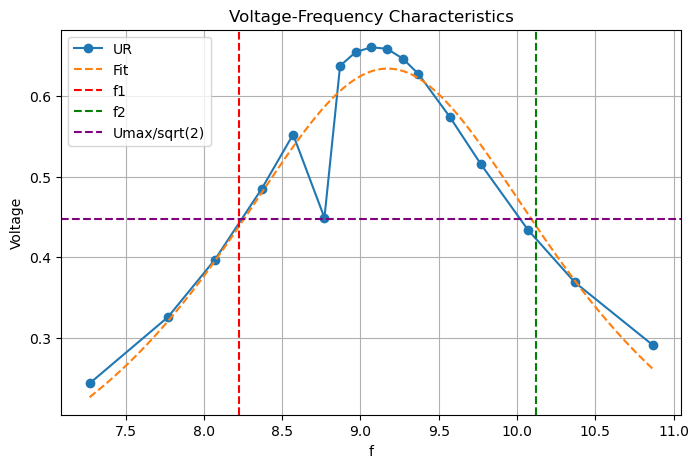
\includegraphics[width=0.8\textwidth]{output3.png}
    \caption{ $\mathrm{C}_1=0.01 \mu \mathrm{~F}, \mathrm{R}_1=200 \Omega$}
    \label{fig:diff_circuit}
\end{figure}

\subsection{C1 = 0.01µ F, R2 = 1 KΩ}
选 $\mathrm{C}_1=0.01 \mu \mathrm{~F}, \mathrm{R}_2=1 \mathrm{~K} \Omega$ ,重复步骤 2,3 的测量过程

\begin{figure}[H]
    \centering
    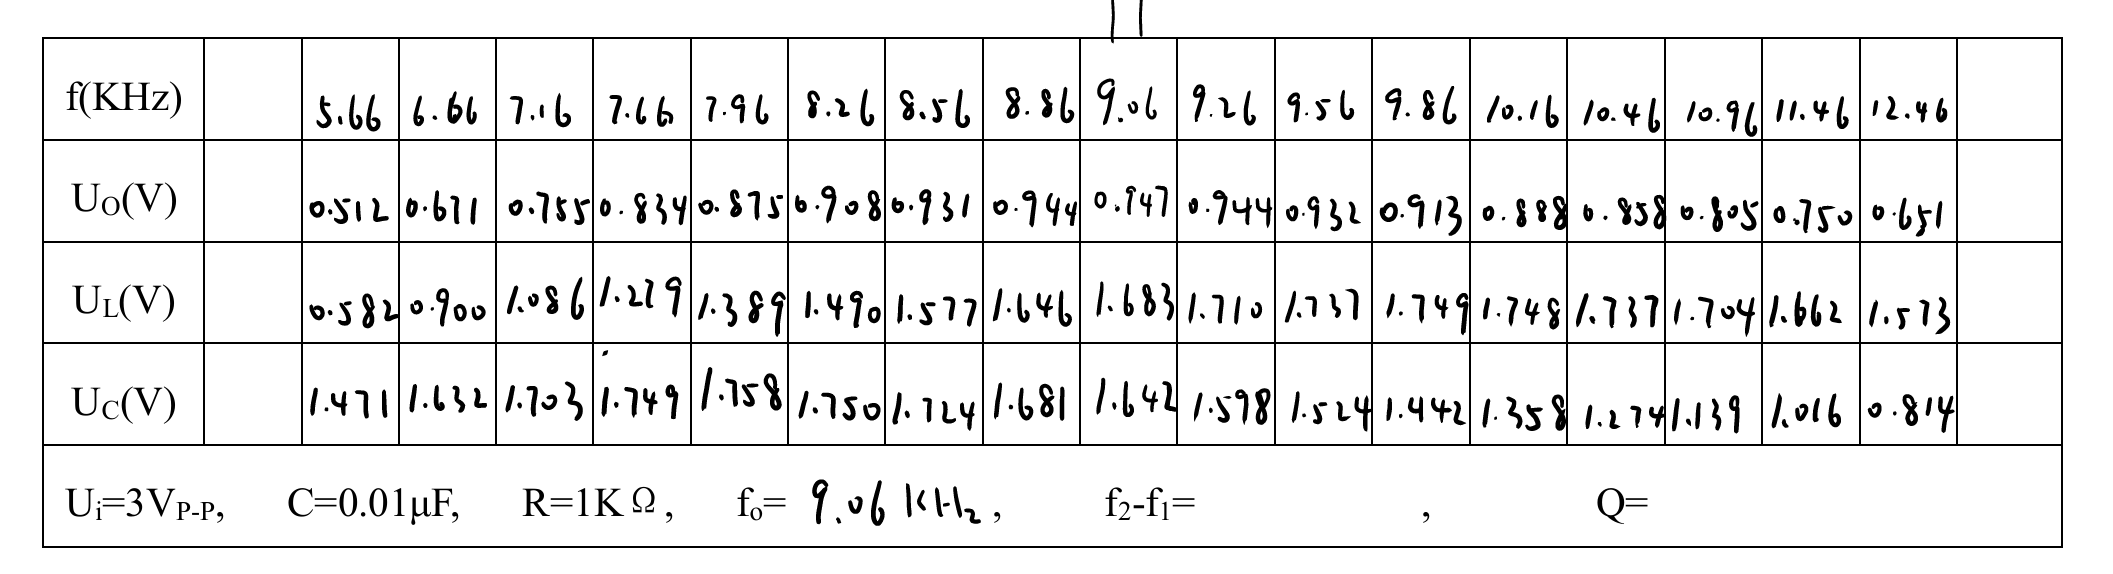
\includegraphics[width=\textwidth]{img5.png}
    \caption{  $\mathrm{C}_1=0.01 \mu \mathrm{~F}, \mathrm{R}_2=1 \mathrm{~K} \Omega$}
    \label{fig:diff_circuit}
\end{figure}
\subsubsection{第一种方法测 Q 值}
根据公式 $\mathrm{Q}=\frac{U_L}{U_o}=\frac{U_C}{U_o}$ 测定, $\mathrm{Q}=\frac{U_L}{U_o}=\frac{U_C}{U_o}=1.68/0.947=1.774$
\subsubsection{通频带宽法 Q 值}
$\mathrm{U}_{\mathrm{i}}=3 \mathrm{~V}_{\mathrm{P}-\mathrm{P}}, \quad \mathrm{C}=0.01 \mu \mathrm{~F}, \quad \mathrm{R}=1 \mathrm{~K} \Omega, \quad \mathrm{f}_0=9.06 \mathrm{k}  \mathrm{Hz}$

$f1 = 6.47 \mathrm{kHz}\quad f2 = 12.09 \mathrm{kHz} \quad \mathrm{f}_2-\mathrm{f}_1=5.62\mathrm{kHz}\quad, \quad \mathrm{Q}= 1.65$

\begin{figure}[H]
    \centering
    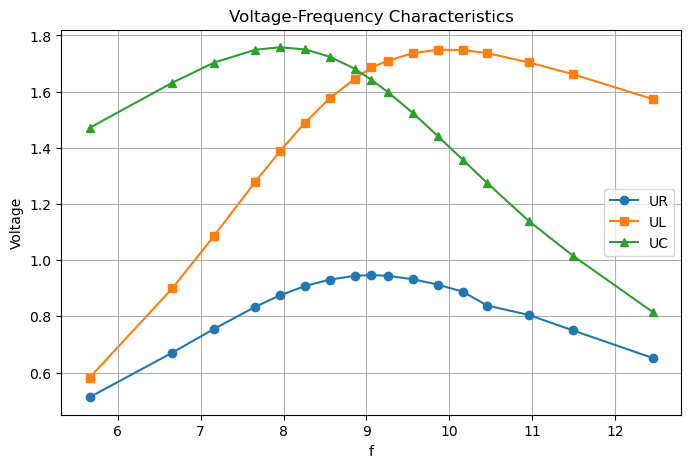
\includegraphics[width=0.8\textwidth]{output2.png}
    \caption{ $\mathrm{C}_1=0.01 \mu \mathrm{~F}, \mathrm{R}_1=1k \Omega$}
    \label{fig:diff_circuit}
\end{figure}
\begin{figure}[H]
    \centering
    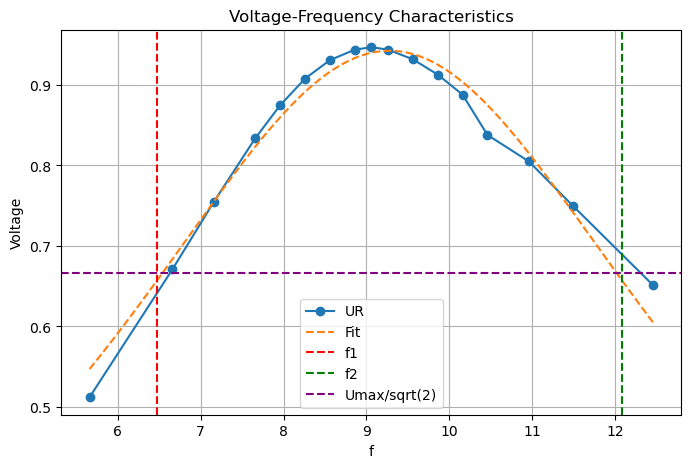
\includegraphics[width=0.8\textwidth]{output4.png}
    \caption{ $\mathrm{C}_1=0.01 \mu \mathrm{~F}, \mathrm{R}_1=1k \Omega$}
    \label{fig:diff_circuit}
\end{figure}

\subsection{不同 R 值时对电路通频带与品质因数的影响}
$$
f_0=2 \pi \omega_0
$$

(f0 谐振频率,$\omega 0$ 谐振角频率)

$$
\begin{aligned}
& \omega_0=\frac{1}{\sqrt{L C}} \\
& Q=\frac{U_L}{U}=\frac{U_C}{U}=\frac{\omega_0 L}{R}=\frac{1}{\omega_0 R C} \\
& \mathbf{Q}=\frac{\mathbf{f}_{\mathrm{e}}}{\mathbf{B W}}
\end{aligned}
$$

(fc 谐振 频率;BW 通频带宽)

$$
\Delta \omega=\omega_2-\omega_1=\frac{\omega_0}{Q}
$$
故 R 越大,Q 值越小,通频带宽越大,电路的选择性越差;R 越小,Q 值越大,通频带宽越小,电路的选择性越好。

\subsection{两种不同的测 Q 值的方法进行比较,分析误差原因}


\subsubsection{误差原因}
\begin{enumerate}
        \item L、C 都不是理想元件,存在着一定的阻抗,导致 UL、Uc 偏高,Q 值偏大
        \item 测量通频带宽度产生误差,导致结果出现偏差。
       
    \end{enumerate} 

测量通频带宽度产生误差,导致结果出现偏差。

\subsection{谐振时,比较输出电压 UO 与输入电压 Ui 是否相等?试分析原因}
谐振时,理论上是相等的,但由于元件参数并非理想参数,尤其是电感元件有一定的等效电阻,而非理想的纯电感。所以实验时,数据与理论值有一定差距。

输出电压 UL $=X L^* I=X L^* U / R$
所以输出电压随着电路中电阻的减小而变大
$\mathrm{Q}=\mathrm{UL} / \mathrm{U}=\mathrm{XL} / \mathrm{R}$ 因此 Q 与 R 有直接关系

对于包含电容和电感及电阻元件的无源一端口网络,其端口可能呈现容性、感性及电阻性,当电路端口的电压 U 和电流 I,出现同相位,电路呈电阻性时。称之为谐振现象,这样的电路,称之为谐振电路。 

谐振的实质是电容中的电场能与电感中的磁场能相互转换,此增彼减,完全补偿。电场能和磁场能的总和时刻保持不变,电源不必与电容或电感往返转换能量,只需供给电路中电阻所消耗的电能。

\subsection{总结、归纳串联谐振电路的特性}

\begin{enumerate}
        \item 无论是电阻的阻值如何变化,电压和电流的波形在不同频率下的变化情况相同,即串联谐振频率的大小与电阻无关,且在发生串联谐振时,电压和电流取得最大值。
        \item 电路的品质因数与电感和电容的值无关,电路的品质因数与电阻成反比。
        \item 串联谐振电路的品质因数 Q 值越大,通频带宽越小,电路的选择性越好。
    \end{enumerate} 



\section{预习思考题 }
\subsection{根据实验线路板给出的元件参数值,估算电路的谐振频率 }

$\mathrm{f}_0=\frac{1}{2 \pi \sqrt{L C}}=     9 \mathrm{k}  \mathrm{Hz}      $

\subsection{改变电路的哪些参数可以使电路发生谐振,电路中 R 的数值是否影响谐振频率值?}
电感$L$和电容$C$,电路中 R 的数值不影响谐振频率值。

\subsection{如何判别电路是否发生谐振?测试谐振点的方案有哪些?}

1、从定义上看可以通过判断串联回路电抗时候为零来判断;

2、在实验中可以通过改变信号源频率,使总阻抗达到最小,此时电路发生谐振。

测试方案:

1、改变 L、C 的数值,测电路中的电流,达到最大值时即为谐振点。

2、改变 L、C 的数值,同时测电路中的 Ul 和 Uc,当 Ul=Uc 时,就为谐振点。

3、改变 L、C 的数值,测电路中的 Ur,当 Ur=Ui 时就为谐振点。



\subsection{电路发生串联谐振时,为什么输入电压不能太大,如果信号源给出 3 V 的电压,电路谐振时,用交流毫伏表测 $\mathrm{U}_{\mathrm{L}}$ 和 $\mathrm{U}_{\mathrm{C}}$ ,应该选择用多大的量限?}

电路发生串联谐振,输入电压不能太大的原因是 UL=Uc=QUi,而 Q 值通常较大,这样,UL、Uc 都会远大于电源电压 Ui,线圈和电容器的绝缘会被击穿而造成损害。

量程为 10V、30V、100V、300V,从大到小依次选择。
\subsection{要提高 $\mathrm{R} 、 \mathrm{~L} 、 \mathrm{C}$ 串联电路的品质因数,电路参数应如何改变?}
$$
Q=\frac{U_L}{U}=\frac{U_C}{U}=\frac{\omega_0 L}{R}=\frac{1}{\omega_0 R C} \\
$$

如果要保证谐振频率不变,最简单的办法就是减小 R 值。若要改变 L 或 C,加大 L,同比例减小 C。

\subsection{本实验在谐振时,对应的 $U_L$ 与 $U_C$ 是否相等?如有差异,原因何在?}
谐振时,理想状态 uc 与 ul 应该相等。但线路总是存在电阻,如有差异就是电阻造成的,尤其是电感的电阻
\section{总结感悟 }
通过这次实验,我学会了如何使用仿真实验平台来查看电压和电流在不同频率下的波形并根据波形找到串联谐振频率,还掌握了通过仿真实验平台来分析不同频率、不通过阻值情况下电压和电流的波形变化情况。而且,这次实验使我对串联谐振的原理以及发生串联谐振时电路具有的特征的理解更加深刻,并熟练掌握了判断电路发生了串联谐振的方法。在此之外,我对串联谐振电路的相关参数的理论计算也变得更加熟练。

\section{参考文献}
\begin{enumerate}
    \item 电子电路实验指导书
    \item 电子电路基础
    \item 电路原理
    \item 电路分析
\end{enumerate} 

\end{document}